\section{Theoretical Analysis}
\label{sec:analysis}

\subsection{Node analysis method ($t < 0$)}
\label{sec:node}

For the time interval $t < 0$, the voltage in the independent voltage source is constant, $v_S(t) = V_S$. As a consequence, to study the circuit in this interval, one can considere it has been on for such an amout of time  that the capacitor is fully charged, which implies that $I_c = 0$.

By analysing the circuit and using KCL and Ohm's Law, it is possible to perform a node analysis and to write an equation for each node as it follows:

\begin{equation}
  \begin{cases}
    (GND) & \frac{V_7}{R_6} + \frac{V_5}{R_4} + \frac{V_2-V_1}{R_1} = 0 \\
    (1) & V_1 = V_S \\
    (2) & -\frac{V_2-V_1}{R_1} - \frac{V_2-V_5}{R_3} + \frac{V_3-V_2}{R_2} = 0 \\
    (3) & I_b - \frac{V_3-V_2}{R_2} = 0 \\
    (5) & V_2-V_5 = V_b \\
    (6) & -I_b - \frac{V_6-V_5}{R_5} - I_c = 0 \\
    (7) & -\frac{V_7}{R_6} + \frac{V_8-V_7}{R_7} = 0 \\
    (8) & V_5-V_8 = V_d
  \end{cases}
\end{equation}

Rearranging these equations and employing the relations $I_b = K_bV_b$ and $V_d = K_dI_d$, it is possible to write the following matrix system:

\begin{equation}
  \begin{bmatrix}
    -\frac{1}{R_1} & \frac{1}{R_1} & 0 & \frac{1}{R_4} & 0 & \frac{1}{R_6} & 0 \\
    1 & 0 & 0 & 0 & 0 & 0 & 0 \\
    \frac{1}{R_1} & -\frac{1}{R_1}-\frac{1}{R_2}-\frac{1}{R_3} & \frac{1}{R_2} & \frac{1}{R_3} & 0 & 0 & 0 \\
    0 & K_b + \frac{1}{R_2} & -\frac{1}{R_2} & -K_b & 0 & 0 & 0 \\
    0 & -K_b & 0 & K_b+\frac{1}{R_5} & -\frac{1}{R_5} & 0 & 0 \\
    0 & 0 & 0 & 0 & 0 & -\frac{1}{R_6}-\frac{1}{R_7} & \frac{1}{R_7} \\
    0 & 0 & 0 & 1 & 0 & \frac{K_d}{R_6} & -1     
  \end{bmatrix}
  \begin{bmatrix}
    V_1 \\
    V_2 \\
    V_3 \\
    V_5 \\
    V_6 \\
    V_7 \\
    V_8
  \end{bmatrix}
  =
  \begin{bmatrix}
    0 \\
    V_S \\
    0 \\
    0 \\
    0 \\
    0 \\
    0
  \end{bmatrix}
\end{equation}

Using {\bf Octave}, it was possible to use the matrix to compute the voltages in all nodes and the currents in all branches. These are presented in Table~\ref{node_res}. 

\begin{table}[H]
  \centering
  \begin{tabular}{|c|c|}
    \hline
        {\bf Name} & {\bf Value} \\
        \hline
        \hline
        $V_2\;(V)$ & $5.070727$ \\ 
\hline
$V_3\;(V)$ & $4.825468$ \\ 
\hline
$V_4\;(V)$ & $4.304579$ \\ 
\hline
$V_5\;(V)$ & $4.860091$ \\ 
\hline
$V_6\;(V)$ & $8.720760$ \\ 
\hline
$V_7\;(V)$ & $-2.939898$ \\ 
\hline
$V_8\;(V)$ & $-1.950198$ \\ 
\hline
$V_b\;(V)$ & $-0.034623$ \\ 
\hline
$I_b\;(V)$ & $-0.000251$ \\ 
\hline
$I_c\;(V)$ & $0.000969$ \\ 
\hline
$V_c\;(V)$ & $7.799989$ \\ 

        \hline
  \end{tabular}
  \caption{Theoretical results}
  \label{node_res}
\end{table}

\subsection{Capacitor behaviour}
\label{sec:Req}

In order to ascertain how the capacitor behaves, the equivalent resistor seen by it was determined. To do this, a tension source was added in lieu of the capacitor, and the response current of the remainder of the circuit was obtained, via node analysis methods.

For this procedure it was considered that $t=0\;s$, at which time the capacitor is fully charged, and so the voltage difference at it's terminals is known from \ref{sec:node} and constant (static analysis). At this time, it is also known that $V_s=0\;V$ - it is the exact time at which the source shifts from constant ($V_s$) to sinusoidal (null).

% Boneco

There are seven unknowns, $V_1$, $V_2$, $V_3$, $V_5$, $V_6$, $V_7$ and $V_8$, and eight nodes. For simplicity's sake, the seven ``easiest'' nodes were considered, that is, including the GND node and discarding node eight (which would require a super-node equation).

\begin{equation}
  \begin{cases}
    (1) & V_1=0 \\
    (2) & \frac{V_1-V_2}{R_1} + \frac{V_5-V_2}{R_3} + \frac{V_3-V_2}{R_2} = 0 \\
    (3) & I_b = \frac{(V_3-V_2)}{R_2} = 0 \\
    (GND) & \frac{V_2-V_1}{R_1} + \frac{V5}{R4} + \frac{V_7}{R_6} = 0 \\
    (5) & V_5-V_8 = V_d \\
    (6) & V_6-V_8 = V_x \\
    (7) & -\frac{V_7}{R_6} + \frac{V_8-V_7}{R_7} = 0
  \end{cases}
\end{equation}

Rearranging these equations and employing the relations $I_b = K_bV_b$ and $V_d = K_dI_d$, it is possible to write the following matrix system:

\begin{equation}
  \begin{bmatrix}
    1 & 0 & 0 & 0 & 0 & 0 & 0 \\
    \frac{1}{R_1} & -\frac{1}{R_1}-\frac{1}{R_2}-\frac{1}{R_3} & \frac{1}{R_2} & \frac{1}{R_3} & 0 & 0 & 0 \\
    0 & K_b + \frac{1}{R_2} & -\frac{1}{R_2} & -K_b & 0 & 0 & 0 \\
    -\frac{1}{R_1} & \frac{1}{R_1} & 0 & \frac{1}{R_4} & 0 &\frac{1}{R_6} & 0 \\
    0 & 0 & 0 & 1 & 0 & \frac{K_d}{R_6} & -1 \\
    0 & 0 & 0 & 0 & 1 & 0 & -1 \\
    0 & 0 & 0 & 0 & 0 & -\frac{1}{R_6}-\frac{1}{R_7} & \frac{1}{R_7}
  \end{bmatrix}
  \begin{bmatrix}
    V_1 \\
    V_2 \\
    V_3 \\
    V_5 \\
    V_6 \\
    V_7 \\
    V_8
  \end{bmatrix}
  =
  \begin{bmatrix}
    0 \\
    0 \\
    0 \\
    0 \\
    0 \\
    V_x \\
    0
  \end{bmatrix}
\end{equation}

The results obtained by solving this system using \textbf{Octave} were as follows:

\begin{table}[H]
  \centering
  \begin{tabular}{|c|c|}
    \hline
        {\bf Name} & {\bf Value} \\
        \hline
        \hline
        \input{../mat/nodeReq}
        \hline
  \end{tabular}
  \caption{Theoretical results}
\end{table}

By applying KCL to node 6, $I_x$ can be calculated:

\begin{equation}
  I_x = I_b - \frac{V_5-V_6}{R_5} = K_b \cdot (V_2-V_5) - \frac{V_5-V_6}{R_5} 
\end{equation}

$R_{eq}$ is then obtained from Ohm's Law:

\begin{equation}
  R_{eq} = \frac{V_x}{I_x}
\end{equation}

\begin{table}[H]
  \centering
  \begin{tabular}{|c|c|}
    \hline
        {\bf Name} & {\bf Value} \\
        \hline
        \hline
        \input{../mat/nodeReq2}
        \hline
  \end{tabular}
  \caption{Theoretical results}
\end{table}

As expected, the current value $I_x$ is negative, thus making $P_x$ negative (the current going through $V_x$ is $-I_x$): the voltage source supplies energy to the circuit. We can then reduce the capacitor's behaviour to:

\begin{figure}[H]
  \centering
  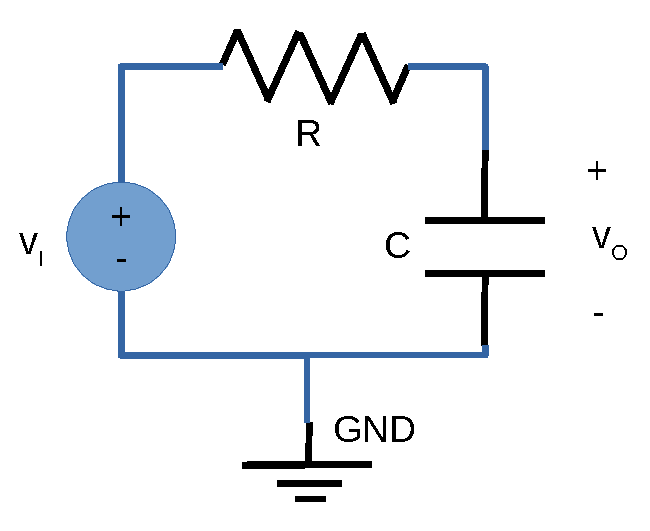
\includegraphics[width=0.6\linewidth]{rc.pdf}
  \caption{Equivalent RC circuit}
  \label{rc_fig}
\end{figure}

In order to confirm the above results do not depend on the potencial difference at the capacitor terminals ($V$), it was also solved using a symbolic package in \textbf{Octave}, which determined:

\begin{table}[H]
  \centering
  \begin{tabular}{|c|c|}
    \hline
        {\bf Name} & {\bf Value} \\
        \hline
        \hline
        \input{../mat/nodeReqb}
        \hline
  \end{tabular}
  \caption{Symbolic solution}
  \label{sym}
\end{table}

It is then true that, no matter $v_c(t)=v_6(t)-v_8(t)$, as the capacitor discharges, all nodes have null potential except for $v_6(t)$.

\subsubsection{Natural solution}

The natural solution of the capacitor behaviour is obtained by considering $v_x(t\geq0)=0$ and $v(0)=V_x$, where $v$ is as depicted in Figure~\ref{rc_fig}. From Table \ref{sym}, we can safely say that $v_8(t)=0\;V$ and $v(t)=v_6(t)\;V$ for the natural response (that is, with $v_s=0\;V$). It is known that:

\begin{equation}
  \begin{cases}
    KVL: & v(t) + R_{eq} \cdot i(t) = 0 \\
    Capacitor: & i(t) = C \cdot \frac{dv(t)}{dt}
  \end{cases}
  \label{sis}
\end{equation}

A first order linear equation arises from \ref{sis}, which can be readily solved:

\begin{equation}
  RC \cdot \frac{dv(t)}{dt} + v(t) = 0 \Rightarrow v(t) = Ae^{-\frac{t}{RC}}
\end{equation}

Applying the initial condition:

\begin{equation}
  v(0) = A = V_x
\end{equation}

The natural solution is:

\begin{equation}
  \label{nat_sol} v(t) =
  \begin{cases}
    V_x & \mbox{if } t \leq 0 \\
    V_xe^{-\frac{t}{RC}} & \mbox{if } t > 0
  \end{cases}
\end{equation}

\begin{figure}[H]
  \centering
  \includegraphics[width=0.8\linewidth]{natural.eps}
  \caption{Natural response}
  \label{fig:nat}
\end{figure}

\subsubsection{Forced solution}
